\part{Outils pour les statistiques}

\section{Paramètres d'une série discrète}\label{paramstats}

\subsection{Idée}

\begin{tipblock}
\cmaj{3.10c} L'idée est de proposer une commande pour déterminer les paramètres d'une série statistique discrète.

Le code se charge de calculer les paramètres (min, q1, méd, q3, max) et de les stocker dans des macros réutilisables.
\end{tipblock}

\begin{PresCodeTexPL}{listing only}
\DeterminerParamStats(*){liste}[\macromin]...[\macromax]
\end{PresCodeTexPL}

\subsection{Arguments, exemples}

\begin{cautionblock}
La version étoilée permet de spécifier que la liste est donnée sous la forme \ctex{val/eff1,val2/eff2,...}, sinon la liste est à donner sous forme brute \ctex{val1,val2,...}.

\smallskip

Les (5) macros par défaut sont 

\begin{itemize}
	\item la macro \Cle{\textbackslash monmin} pour stocker min ;
	\item la macro \Cle{\textbackslash monquartileun} pour stocker q1 ;
	\item la macro \Cle{\textbackslash mamediane} pour stocker méd ;
	\item la macro \Cle{\textbackslash monquartiletrois} pour stocker q3 ;
	\item la macro \Cle{\textbackslash monmax} pour stocker max.
\end{itemize}
\vspace*{-\baselineskip}\leavevmode
\end{cautionblock}

\begin{PresCodePL}{}
%avec des données brutes
\def\listedonnees{0.7426,0.7429,0.7435,0.7448,0.7456,0.7478,0.7478,0.748,0.7487,0.7494,0.7494,0.7496}

\DeterminerParamStats{\listedonnees}
\monmin/\monquartileun/\mamediane/\monquartiletrois/\monmax
\end{PresCodePL}

\begin{PresCodePL}{}
%avec des données/effectifs
\def\listedonneesregroup{2/25,3/18,4/17,5/10,6/5,7/20,8/2}

\DeterminerParamStats*{\listedonneesregroup}
La valeur minimale est \monmin.\\
La médiane est \mamediane.\\
Le premier quartile est \monquartileun.\\
Le troisième quartile est \monquartiletrois.\\
La valeur maximale est \monmax.
\end{PresCodePL}

\newpage

\section{Paramètres d'une régression linéaire par la méthode des moindres carrés}\label{reglin}

\subsection{Idée}

\begin{tipblock}
L'idée est d'utiliser une commande qui va permettre de calculer les paramètres principaux d'un régression linéaire par la méthode des moindres carrés.

Le package \ctex{pgfpots} permet de le faire nativement, mais le moteur de calculs de \textsf{pgf} peut poser souci avec de grandes valeurs, donc ici cela passe par \ctex{xfp} qui permet de \textit{gagner} en précision !

\smallskip

L'idée est que cette macro calcule et stocke les paramètres dans des variables (le nom peut être personnalisé !) pour exploitation ultérieure :

\begin{itemize}
\item en calculs \textit{purs} ;
\item dans un environnement \TikZ{} via \textsf{pgfplots} ou bien en \textit{natif} ;
\item dans un environnement \PSTricks{} ;
\item dans un environnement \hologo{METAPOST} (à vérifier quand même) ;
\item \ldots
\end{itemize}
\vspace*{-\baselineskip}\leavevmode
\end{tipblock}

\begin{PresCodeTexPL}{listing only}
...
\CalculsRegLin[clés]{listeX}{listeY}  %listes avec éléments séparés par des ,
...
\end{PresCodeTexPL}

\begin{noteblock}
La commande \ctex{CalculsRegLin} va définir également des \textsf{macros} pour chaque coefficient, qui de ce fait seront réutilisables après !
\end{noteblock}

\subsection{Commandes}

\begin{cautionblock}
Quelques \Cle{Clés} sont disponibles pour cette commande, essentiellement pour \textit{renommer} les paramètres :

\begin{itemize}
\item la clé \Cle{NomCoeffa} qui permet de définir la variable qui contiendra $a$ ;\hfill{}défaut \Cle{COEFFa}
\item la clé \Cle{NomCoeffb} qui permet de définir la variable qui contiendra $b$ ;\hfill{}défaut \Cle{COEFFb}
\item la clé \Cle{NomCoeffr} qui permet de définir la variable qui contiendra $r$ ;\hfill{}défaut \Cle{COEFFr}
\item la clé \Cle{NomCoeffrd} qui permet de définir la variable qui contiendra $r^2$ ;\hfill{}défaut \Cle{COEFFrd}
\item la clé \Cle{NomXmin} qui permet de définir la variable qui contiendra $x_{\text{min}}$ ;\hfill{}défaut \Cle{LXmin}
\item la clé \Cle{NomXmax} qui permet de définir la variable qui contiendra $x_{\text{max}}$.\hfill{}défaut \Cle{LXmax}
\end{itemize}
\vspace*{-\baselineskip}\leavevmode
\end{cautionblock}

\begin{PresCodeTexPL}{listing only}
%les espaces verticaux n'ont pas été écrits ici
\def\LLX{1994,1995,1996,1997,1998,1999,2000,2001,2002,2004,2005,2006,2007,2008, 2009,2010}
\def\LLY{1718,1710,1708,1700,1698,1697,1691,1688,1683,1679,1671,1670,1663,1661, 1656,1649}
\CalculsRegLin{\LLX}{\LLY}
\end{PresCodeTexPL}

\begin{PresCodeTexPL}{listing only}
%vérif des calculs (noms non modifiables...)
Liste des X := \showitems\LX.
Liste des Y := \showitems\LY.
Somme des X := \LXSomme{} et somme des Y := \LYSomme.
Moyenne des X := \LXmoy{} et moyenne des Y := \LYmoy.
Variance des X := \LXvar{} et variance des Y := \LYvar{}
Covariance des X/Y := \LXYvar.
%les coefficients, avec des noms modifiables !
Min des X := \LXmin{} et Max des X := \LXmax.
Coefficient $a=\COEFFa$.
Coefficient $b=\COEFFb$.
Coefficient $r=\COEFFr$.
Coefficient $r^2=\COEFFrd$.
\end{PresCodeTexPL}

\begin{PresCodeSortiePL}{text only}
\def\LLX{1994,1995,1996,1997,1998,1999,2000,2001,2002,2004,2005,2006,2007,2008,2009,2010}
\def\LLY{1718,1710,1708,1700,1698,1697,1691,1688,1683,1679,1671,1670,1663,1661,1656,1649}
\CalculsRegLin{\LLX}{\LLY}

Liste des X := \showitems\LX.

\smallskip

Liste des Y := \showitems\LY.

\smallskip

Somme des X := \LXSomme{} et somme des Y := \LYSomme.

\smallskip

Moyenne des X := \LXmoy{} et moyenne des Y := \LYmoy.

\smallskip

Variance des X := \LXvar{} et variance des Y := \LYvar{}

\smallskip

Covariance des X/Y := \LXYvar.

\smallskip

Min des X := \LXmin{} et Max des X := \LXmax.

\smallskip

Coefficient $a=\COEFFa$.\tabto{0.5\textwidth}Coefficient $b=\COEFFb$.

%\smallskip
%
%Coefficient $b=\COEFFb$.

\smallskip

Coefficient $r=\COEFFr$.\tabto{0.5\textwidth}Coefficient $r^2=\COEFFrd$.

%\smallskip
%
%Coefficient $r^2=\COEFFrd$.
\end{PresCodeSortiePL}

\begin{noteblock}
\hfill~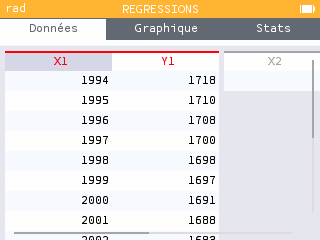
\includegraphics[height=3cm]{./graphics/pl-doc-stats_a}~~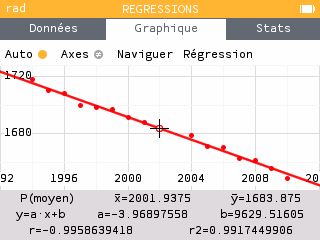
\includegraphics[height=3cm]{./graphics/pl-doc-stats_b}~~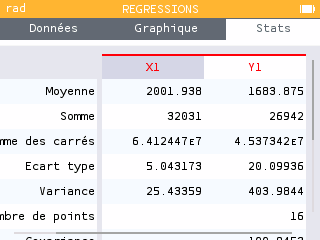
\includegraphics[height=3cm]{./graphics/pl-doc-stats_c}~~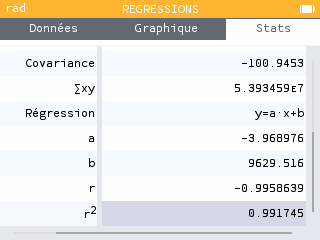
\includegraphics[height=3cm]{./graphics/pl-doc-stats_c2}\hfill~
\end{noteblock}

\begin{noteblock}
Les \textsf{macros} qui contiennent les paramètres de la régression sont donc réutilisables, en tant que nombres réels, donc exploitables par \ctex{siunitx} et \ctex{xfp} pour affichage \textit{fin} ! Ci-dessous un exemple permettant de visualiser tout cela.
\end{noteblock}

\begin{PresCodeTexPL}{listing only}
%les espaces verticaux n'ont pas été écrits ici
\def\LstX{0,1,3,4,5,6}
\def\LstY{-35,-37.4,-37.7,-39.9,-39,-39.6}
%on lance les calculs et on change le nom des "macros-résultats"
\CalculsRegLin[NomCoeffa=TESTa,NomCoeffb=TESTb,NomCoeffr=TESTr,NomCoeffrd=TESTrd,%
           NomXmin=TESTmin,NomXmax=TESTmax]{\LstX}{\LstY}
%commandes complémentaires
\DeclareDocumentCommand\arrond{ s O{3} m }{% * signe / précision / nb
	\IfBooleanTF{#1}{\num[print-implicit-plus]{\fpeval{round(#3,#2)}}} {\num{\fpeval{round(#3,#2)}}}
}
%paramètres
Les valeurs extr. de X sont \TESTmin{} et \TESTmax. Une éq. est $y=\arrond[3]{\TESTa}x \arrond*[3]{\TESTb}$.
Le coeff. de corrélation est $r=\arrond[4]{\TESTr}$, et son carré est $r^2=\arrond[4]{\TESTrd}$.
\end{PresCodeTexPL}

\begin{PresCodeSortiePL}{text only}
\def\LstX{0,1,3,4,5,6}\def\LstY{-35,-37.4,-37.7,-39.9,-39,-39.6}
\CalculsRegLin[NomCoeffa=TESTa,NomCoeffb=TESTb,NomCoeffr=TESTr,NomCoeffrd=TESTrd,NomXmin=TESTmin,NomXmax=TESTmax]{\LstX}{\LstY}
\DeclareDocumentCommand\arrond{ s O{3} m }{
	\IfBooleanTF{#1}{\num[print-implicit-plus]{\fpeval{ceil(#3,#2)}}}
		{\num{\fpeval{round(#3,#2)}}}
}

Les valeurs extrêmes de $x$ sont \TESTmin{} et \TESTmax. Une équation de la droite de régression de $y$ en $x$ est 

\hfill$y=\arrond[3]{\TESTa}x \arrond*[3]{\TESTb}$.\hfill~

\smallskip

Le coefficient de corrélation linéaire est $r=\arrond[4]{\TESTr}$, et son carré est $r^2=\arrond[4]{\TESTrd}$.
\end{PresCodeSortiePL}

\begin{noteblock}
\hfill~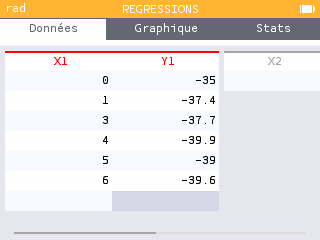
\includegraphics[height=3cm]{./graphics/pl-doc-stats_d}~~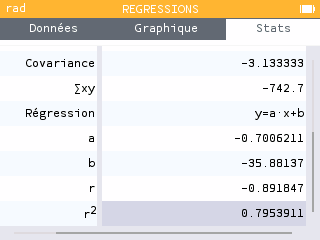
\includegraphics[height=3cm]{./graphics/pl-doc-stats_e}\hfill~
\end{noteblock}

\subsection{Intégration dans un environnement \TikZ}

\begin{noteblock}
La commande étant \og autonome \fg{}, elle va pouvoir être intégrée dans des environnements graphiques pour permettre un tracé \textit{facile} de la droite de régression.
\end{noteblock}

\begin{PresCodeTexPL}{listing only}
\begin{tikzpicture}
\begin{axis}[options des axes, non présentées ici...]
		\addplot[teal, only marks] table{
				X Y
				1994 1718 1995 1710 1996 1708 1997 1700 1998 1698 1999 1697 2000 1691 2001 1688
				2002 1683 2004 1679 2005 1671 2006 1670 2007 1663 2008 1661 2009 1656 2010 1649
			};
		\def\LLX{1994,1995,1996,1997,1998,1999,2000,2001,2002,2004,2005,2006,2007,2008, 2009,2010}
		\def\LLY{1718,1710,1708,1700,1698,1697,1691,1688,1683,1679,1671,1670,1663,1661, 1656,1649}
		\CalculsRegLin{\LLX}{\LLY}
		\addplot [thick,orange,domain=\LXmin:\LXmax,samples=2]{\COEFFa*x+\COEFFb};
		\addlegendentry{$y = \fpeval{round(\COEFFa,3)}\,x + \fpeval{round(\COEFFb,3)}$};
		\addlegendentry{$R^2=\fpeval{round(\COEFFrd,5)}$};
	\end{axis}
\end{tikzpicture}
\end{PresCodeTexPL}

\begin{PresCodeSortiePL}{text only}
\begin{tikzpicture}
\begin{axis}[
		/pgf/number format/.cd,
		use comma,
		xmin = 1992, xmax = 2012,
		ymin = 1640, ymax = 1730,
		width = 0.7\textwidth,
		height = 0.35\textwidth,
		xtick distance = 2,
		ytick distance = 10,
		grid = both,
		minor tick num = 1,
		major grid style = {lightgray},
		minor grid style = {lightgray!25},
		xlabel = {\small Année ($x$)},
		ylabel = {\small Altitude du glacier (en m) ($y$)},
		x tick label style={/pgf/number format/.cd, set thousands separator={}},
		y tick label style={/pgf/number format/.cd, set thousands separator={}},
		legend cell align = {left},
		legend pos = north east
		]
		\addplot[teal, only marks] table{
				X Y
				1994 1718
				1995 1710
				1996 1708
				1997 1700
				1998 1698
				1999 1697
				2000 1691
				2001 1688
				2002 1683
				2004 1679
				2005 1671
				2006 1670
				2007 1663
				2008 1661
				2009 1656
				2010 1649
			};
		\def\LLX{1994,1995,1996,1997,1998,1999,2000,2001,2002,2004,2005,2006,2007,2008,2009,2010}
		\def\LLY{1718,1710,1708,1700,1698,1697,1691,1688,1683,1679,1671,1670,1663,1661,1656,1649}
		\CalculsRegLin{\LLX}{\LLY}
		\addplot [thick,orange,domain=\LXmin:\LXmax,samples=2]{\COEFFa*x+\COEFFb};
		\addlegendentry{$y = \fpeval{round(\COEFFa,3)}\,x + \fpeval{round(\COEFFb,3)}$};
		\addlegendentry{$R^2=\fpeval{round(\COEFFrd,5)}$};
	\end{axis}
\end{tikzpicture}
\end{PresCodeSortiePL}

\begin{noteblock}
Il existe également une commande auxiliaire, \ctex{PointsRegLin} pour afficher le nuage de points avec quelques options, dans un environnement \TikZ{} classique (sans \textsf{pgfplot})\ldots
\end{noteblock}

\begin{PresCodeTexPL}{listing only}
...
\begin{tikzpicture}[<options>]
...
\PointsRegLin[clés]{listeX}{listeY}
...
\end{tikzpicture}
\end{PresCodeTexPL}

\begin{cautionblock}
Quelques \Cle{Clés} sont disponibles pour cette commande, essentiellement pour la mise en forme du nuage :

\begin{itemize}
\item la clé \Cle{Couleur} pour la couleur des points du nuage ;\hfill{}défaut \Cle{teal}
\item la clé \Cle{Taille} pour la taille des points (type \textit{cercle}) ;\hfill{}défaut \Cle{2pt}
\item la clé \Cle{Ox} pour spécifier la valeur initiale Ox (si changement d'origine) ;\hfill{}défaut \Cle{0}
\item la clé \Cle{Oy} pour spécifier la valeur initiale Oy (si changement d'origine).\hfill{}défaut \Cle{0}
\end{itemize}
\vspace*{-\baselineskip}\leavevmode
\end{cautionblock}

\begin{PresCodeTexPL}{listing only}
\begin{tikzpicture}[x=0.5cm,y=0.05cm]
\draw[xstep=1,ystep=5,lightgray!50,very thin] (0,0) grid (20,100);
\draw[xstep=2,ystep=10,lightgray,thin] (0,0) grid (20,100);
\draw[thick,->,>=latex] (0,0)--(20,0) ;
\draw[thick,->,>=latex] (0,0)--(0,100) ;
\foreach \x in {1992,1994,...,2010} \draw[thick] ({\x-1992},4pt)--({\x-1992},-4pt) node[below] {$\x$} ;
\foreach \y in {1640,1650,...,1730} \draw[thick] (4pt,{\y-1640})--(-4pt,{\y-1640}) node[left] {$\y$} ;
\def\LLX{1994,1995,1996,1997,1998,1999,2000,2001,2002,2004,2005,2006,2007,2008, 2009,2010}
\def\LLY{1718,1710,1708,1700,1698,1697,1691,1688,1683,1679,1671,1670,1663,1661, 1656,1649}
\def\Ox{1992}\def\Oy{1640}
\CalculsRegLin{\LLX}{\LLY}
\PointsRegLin[Ox=1992,Oy=1640,Couleur=blue,Taille=3pt]{\LLX}{\LLY}
\draw[orange,very thick,samples=2,domain=\LXmin:\LXmax] plot ({\x-\Ox},{\COEFFa*(\x)+\COEFFb-\Oy}) ;
\matrix [draw,fill=white,below left] at (current bounding box.north east) {
		\node {$y=\num{\fpeval{round(\COEFFa,3)}}\,x+\num{\fpeval{round(\COEFFb,3)}}$} ; \\
		\node {$R^2=\num{\fpeval{round(\COEFFrd,5)}}$} ; \\
	};
\end{tikzpicture}
\end{PresCodeTexPL}

\begin{PresCodeSortiePL}{text only}
\begin{tikzpicture}[x=0.5cm,y=0.05cm]
\draw[xstep=1,ystep=5,lightgray!50,very thin] (0,0) grid (20,100);
\draw[xstep=2,ystep=10,lightgray,thin] (0,0) grid (20,100);
\draw[thick,->,>=latex] (0,0)--(20,0) ;
\draw[thick,->,>=latex] (0,0)--(0,100) ;
\foreach \x in {1992,1994,...,2010} \draw[thick] ({\x-1992},4pt)--({\x-1992},-4pt) node[below] {$\x$} ;
\foreach \y in {1640,1650,...,1730} \draw[thick] (4pt,{\y-1640})--(-4pt,{\y-1640}) node[left] {$\y$} ;
\def\LLX{1994,1995,1996,1997,1998,1999,2000,2001,2002,2004,2005,2006,2007,2008,2009,2010}
\def\LLY{1718,1710,1708,1700,1698,1697,1691,1688,1683,1679,1671,1670,1663,1661,1656,1649}
\def\Ox{1992}\def\Oy{1640}
\CalculsRegLin{\LLX}{\LLY}
\PointsRegLin[Ox=1992,Oy=1640,Couleur=blue,Taille=3pt]{\LLX}{\LLY}
\draw[orange,very thick,samples=2,domain=\LXmin:\LXmax] plot ({\x-\Ox},{\COEFFa*(\x)+\COEFFb-\Oy}) ;
\matrix [draw,fill=white,below left] at (current bounding box.north east) {
		\node {$y=\num{\fpeval{round(\COEFFa,3)}}\,x + \num{\fpeval{round(\COEFFb,3)}}$} ; \\
		\node {$R^2=\num{\fpeval{round(\COEFFrd,5)}}$} ; \\
	};
\end{tikzpicture}
\end{PresCodeSortiePL}

\newpage

\section{Statistiques à deux variables}\label{statsdeuxvars}

\subsection{Idées}

\begin{tipblock}
L'idée est de \textit{prolonger} le paragraphe précédent pour proposer un environnement \TikZ{} adapté à des situations venant de statistiques à deux variables.

\smallskip

Un des soucis pour ces situations est le fait que le repère dans lequel on travaille n'a pas forcément pour origine $(0;0)$.

De ce fait -- pour éviter des erreurs de \ctex{dimension too large} liées à \TikZ{} -- il faut \textit{décaler les axes} pour se ramener à une origine en $O$.

\smallskip

Le code, intimement lié à un environnement \ctex{tikzpicture}, va donc :

\begin{itemize}
\item préciser les informations utiles comme \ctex{xmin}, \ctex{xmax}, \ctex{Ox}, \ctex{xgrille}, etc
\item proposer des commandes (sans se soucier des \textit{translations} !) pour :
\begin{itemize}
		\item tracer une grille (principale et/ou secondaire) ;
		\item tracer les axes (avec légendes éventuelles) et éventuellement les graduer ;
	\end{itemize}
\end{itemize}

En utilisant les commandes de \textsf{régression linéaire} du paragraphe précédent, il sera de plus possible (sans calculs !) de :

\begin{itemize}
\item représenter le nuage de points ;
\item placer le point moyen ;
\item tracer la droite d'ajustement (obtenue par \ctex{ProfLycee}) ou une autre courbe.
\end{itemize}
\vspace*{-\baselineskip}\leavevmode
\end{tipblock}

\begin{noteblock}
Le package \ctex{pgfplots} peut être utilisé pour traiter ce genre de situation, mais ne l'utilisant pas, j'ai préféré préparer des \textsf{macros} permettant de s'affranchir de ce package (est-ce pertinent, ça c'est une autre question\ldots).
\end{noteblock}

\begin{PresCodeTexPL}{listing only}
%Listes et calculs
\def\LLX{1994,1995,1996,1997,1998,1999,2000,2001,2002,2004,2005,2006,2007,2008, 2009,2010}
\def\LLY{1718,1710,1708,1700,1698,1697,1691,1688,1683,1679,1671,1670,1663,1661, 1656,1649}
\CalculsRegLin{\LLX}{\LLY}
\end{PresCodeTexPL}

\begin{PresCodeTexPL}{listing only}
%tracé (simple), les options seront présentées juste après
\begin{tikzpicture}%
[x=0.5cm,y=0.1cm,                                             %unités
Ox=1992,xmin=1992,xmax=2012,xgrille=2,xgrilles=1,             %axe Ox
Oy=1640,ymin=1640,ymax=1730,ygrille=10,ygrilles=5]            %axe Oy
\GrilleTikz \AxesTikz                                         %grilles et axes
\AxexTikz[Annee]{1992,1994,...,2010}                          %axeOx
\AxeyTikz{1640,1650,...,1720}                                 %axeOy
\NuagePointsTikz{\LLX}{\LLY}                                  %nuage
\CourbeTikz[line width=1.25pt,CouleurVertForet,samples=2]%
	{\COEFFa*\x+\COEFFb}{\LXmin:\LXmax}                       %droite de régression
\PointMoyenTikz                                               %point moyen
\end{tikzpicture}
\end{PresCodeTexPL}

\begin{PresCodeTexPL}{listing only}
%tracé avec options fenêtre par défaut
\begin{tikzpicture}%
[....]                                                              %paramètres
\FenetreSimpleTikz<Annee>{1992,1994,...,2010}{1640,1650,...,1720}   %fenêtre "simple"
\NuagePointsTikz{\LLX}{\LLY}                                        %nuage
\CourbeTikz[line width=1.25pt,CouleurVertForet,samples=2]%
	{\COEFFa*\x+\COEFFb}{\LXmin:\LXmax}                             %droite de régression
\PLnuageptmoy                                                       %point moyen
\end{tikzpicture}
\end{PresCodeTexPL}

\begin{PresCodeSortiePL}{text only}
\def\LLX{1994,1995,1996,1997,1998,1999,2000,2001,2002,2004,2005,2006,2007,2008,2009,2010}
\def\LLY{1718,1710,1708,1700,1698,1697,1691,1688,1683,1679,1671,1670,1663,1661,1656,1649}
\CalculsRegLin{\LLX}{\LLY}

\begin{tikzpicture}[x=0.5cm,y=0.1cm,Ox=1992,xmin=1992,xmax=2012,xgrille=2,xgrilles=1,Oy=1640,ymin=1640,ymax=1730,ygrille=10,ygrilles=5]
\GrilleTikz \AxesTikz
\AxexTikz[Annee]{1992,1994,...,2010}
\AxeyTikz{1640,1650,...,1720}
\NuagePointsTikz{\LLX}{\LLY}
\CourbeTikz[line width=1.25pt,CouleurVertForet,samples=2]{\COEFFa*\x+\COEFFb}{\LXmin:\LXmax}
\PointMoyenTikz
\end{tikzpicture}
\end{PresCodeSortiePL}

\subsection{Commandes, clés et options}

\begin{noteblock}
Les \Cle{paramètres} nécessaires à la bonne utilisation des commandes suivantes sont à déclarer directement dans l'environnement \ctex{tikzpicture}, seules les versions \og x \fg{}  sont présentées ici:

\begin{itemize}
\item \Cle{xmin}, stockée dans \ctex{\textbackslash{}xmin} ;\hfill{}défaut \Cle{-3}
\item \Cle{xmax}, stockée dans \ctex{\textbackslash{}xmax} ;\hfill{}défaut \Cle{3}
\item \Cle{Ox}, stockée dans \ctex{\textbackslash{}axexOx}, origine de l'axe $(Ox)$ ;\hfill{}défaut \Cle{0}
\item \Cle{xgrille}, stockée dans \ctex{\textbackslash{}xgrille}, graduation principale ;\hfill{}défaut \Cle{1}
\item \Cle{xgrilles}, stockée dans \ctex{\textbackslash{}xgrilles}, graduation secondaire.\hfill{}défaut \Cle{0.5}
\end{itemize}

La fenêtre d'affichage (de sortie) sera donc \textit{portée} par le rectangle de coins $(\text{xmin};\text{ymin})$ et $(\text{xmax};\text{ymax})$ ; ce qui correspond en fait à la fenêtre \TikZ{} \textit{portée} par le rectangle de coins $(\text{xmin-Ox};\text{ymin-Oy})$ et $(\text{xmax-Ox};\text{ymax-Oy})$.

\smallskip

Les commandes ont -- pour certaines -- pas mal de \Cle{clés} pour des réglages fins, mais dans la majorité des cas elles ne sont pas forcément \textit{utiles}.
\end{noteblock}

\begin{noteblock}
Pour illustrer les commandes et options de ce paragraphe, la base sera le graphique présenté précédemment.
\end{noteblock}

\begin{PresCodeTexPL}{listing only}
%...code tikz
\GrilleTikz[options][options grille ppale][options grille second.]
\end{PresCodeTexPL}

\begin{cautionblock}
Cette commande permet de tracer une grille principale et/ou une grille secondaire :

\begin{itemize}
\item les premières \Cle{clés} sont les booléens \Cle{Affp} et \Cle{Affs} qui affichent ou non les grilles ;

\hfill~défaut \Cle{true}
\item les options des grilles sont en \TikZ. \hfill~défaut \Cle{thin,lightgray} et \Cle{very thin,lightgray}
\end{itemize}
\vspace*{-\baselineskip}\leavevmode
\end{cautionblock}

\begin{PresCodeTexPL}{listing only}
\begin{tikzpicture}%
[x=0.3cm,y=0.06cm,%
Ox=1992,xmin=1992,xmax=2012,xgrille=2,xgrilles=1,%
Oy=1640,ymin=1640,ymax=1730,ygrille=10,ygrilles=5]
\GrilleTikz
\end{tikzpicture}
~~
\begin{tikzpicture}%
[x=0.3cm,y=0.06cm,%
Ox=1992,xmin=1992,xmax=2012,xgrille=2,xgrilles=1,%
Oy=1640,ymin=1640,ymax=1730,ygrille=10,ygrilles=5]
\GrilleTikz[Affp=false][][orange,densely dotted]
\end{tikzpicture}
\end{PresCodeTexPL}

\begin{PresCodeSortiePL}{text only}
\hfill~
\begin{tikzpicture}%
[x=0.3cm,y=0.06cm,%
Ox=1992,xmin=1992,xmax=2012,xgrille=2,xgrilles=1,%
Oy=1640,ymin=1640,ymax=1730,ygrille=10,ygrilles=5]
\GrilleTikz
\end{tikzpicture}
~~
\begin{tikzpicture}%
[x=0.3cm,y=0.06cm,%
Ox=1992,xmin=1992,xmax=2012,xgrille=2,xgrilles=1,%
Oy=1640,ymin=1640,ymax=1730,ygrille=10,ygrilles=5]
\GrilleTikz[Affp=false][][orange,densely dotted]
\end{tikzpicture}
\hfill~
\end{PresCodeSortiePL}

\begin{PresCodeTexPL}{listing only}
%...code tikz
\AxesTikz[options]
\end{PresCodeTexPL}

\begin{cautionblock}
Cette commande permet de tracer les axes, avec des \Cle{clés} :

\begin{itemize}
\item \Cle{Epaisseur} qui est l'épaisseur des traits ; \hfill~défaut \Cle{1.25pt}
\item \Cle{Police} qui est le style des labels des axes  ; \hfill~défaut \Cle{\textbackslash{}normalsize\textbackslash{}normalfont}
\item \cmaj{2.1.2} \Cle{ElargirOx} qui est le \% l'élargissement \Cle{global} ou \Cle{G/D} de l'axe $(Ox)$ ;

\hfill~défaut \Cle{0/0.05}
\item \cmaj{2.1.2} \Cle{ElargirOy} qui est le \% l'élargissement \Cle{global} ou \Cle{B/H} de l'axe $(Oy)$ ;

\hfill~défaut \Cle{0/0.05}
\item \Cle{Labelx} qui est le label de l'axe $(Ox)$ ; \hfill~défaut \Cle{\${}x\$}
\item \Cle{Labely} qui est le label de l'axe $(Oy)$ ; \hfill~défaut \Cle{\${}y\$}
\item \Cle{AffLabel} qui est le code pour préciser quels labels afficher, entre \Cle{x}, \Cle{y} ou \Cle{xy} ;

\hfill~défaut \Cle{vide}
\item \Cle{PosLabelx} pour la position du label de $(Ox)$ en bout d'axe ; \hfill~défaut \Cle{right}
\item \Cle{PosLabely} pour la position du label de $(Oy)$ en bout d'axe ; \hfill~défaut \Cle{above}
\item \Cle{EchelleFleche} qui est l'échelle de la flèche des axes ; \hfill~défaut \Cle{1}
\item \Cle{TypeFleche} qui est le type de la flèche des axes.\hfill~défaut \Cle{latex}
\end{itemize}
\vspace*{-\baselineskip}\leavevmode
\end{cautionblock}

\begin{PresCodeTexPL}{listing only}
%code tikz
\AxesTikz

%code tikz
\AxesTikz%
	[AffLabel=xy,Labelx={Année},Labely={Altitude},%
	PosLabelx={below right},PosLabely={above left},%
	Police=\small\sffamily]
\end{PresCodeTexPL}

\begin{PresCodeSortiePL}{text only}
\hfill~
\begin{tikzpicture}%
[x=0.3cm,y=0.06cm,%
Ox=1992,xmin=1992,xmax=2012,xgrille=2,xgrilles=1,%
Oy=1640,ymin=1640,ymax=1730,ygrille=10,ygrilles=5]
\AxesTikz
\end{tikzpicture}
~~
\begin{tikzpicture}%
[x=0.3cm,y=0.06cm,%
Ox=1992,xmin=1992,xmax=2012,xgrille=2,xgrilles=1,%
Oy=1640,ymin=1640,ymax=1730,ygrille=10,ygrilles=5]
\AxesTikz%
	[AffLabel=xy,Labelx={Année},Labely={Altitude},%
	PosLabelx={below right},PosLabely={above left},%
	Police=\small\sffamily]
\end{tikzpicture}
\hfill~
\end{PresCodeSortiePL}

%les axes

\begin{PresCodeTexPL}{listing only}
%...code tikz
\AxexTikz[options]{valeurs}
\AxeyTikz[options]{valeurs}
\end{PresCodeTexPL}

\begin{cautionblock}
Ces commande permet de tracer les graduations des axes, avec des \Cle{clés} identiques pour les deux directions :

\begin{itemize}
\item \Cle{Epaisseur} qui est l'épaisseur des graduations ; \hfill~défaut \Cle{1pt}
\item \Cle{Police} qui est le style des labels des graduations ; \hfill~défaut \Cle{\textbackslash{}normalsize\textbackslash{}normalfont}
\item \Cle{PosGrad} qui est la position des graduations par rapport à l'axe ; \hfill~défaut \Cle{below} et \Cle{left}
\item \Cle{HautGrad} qui est la position des graduations (sous la forme \Cle{lgt} ou \Cle{lgta/lgtb}) ;

\hfill~défaut \Cle{4pt}
\item le booléen \Cle{AffGrad} pour afficher les valeurs (formatés avec \ctex{num} donc dépendant de \ctex{sisetup}) des graduations  ; \hfill~défaut \Cle{true}
\item le booléen \Cle{AffOrigine} pour afficher la graduation de l'origine ; \hfill~défaut \Cle{true}
\item le booléen \Cle{Annee} qui permet de ne pas formater les valeurs des graduations (type \textsf{année}). \hfill~défaut \Cle{false}
\end{itemize}
\vspace*{-\baselineskip}\leavevmode
\end{cautionblock}

\begin{PresCodeTexPL}{listing only}
%code tikz
\AxexTikz[Police=\small]{1992,1994,...,2010}
\AxexTikz{1640,1650,...,1720}

%code tikz
\AxeyTikz[Police=\small,Annee,HautGrad=0pt/4pt]{1992,1994,...,2010}
\AxeyTikz[AffGrad=false,HautGrad=6pt]{1640,1650,...,1720}

%des axes fictifs (en gris) sont rajoutés pour la lisibilité du code de sortie
\end{PresCodeTexPL}

\begin{PresCodeSortiePL}{text only}
\hfill~
\begin{tikzpicture}%
[x=0.3cm,y=0.06cm,%
Ox=1992,xmin=1992,xmax=2012,xgrille=2,xgrilles=1,%
Oy=1640,ymin=1640,ymax=1730,ygrille=10,ygrilles=5]
\draw[gray,line width=1.25pt,->,>=latex] ({\xmin-\axexOx},0) -- ({\xmax-\axexOx},0) ;
\draw[gray,line width=1.25pt,->,>=latex] (0,{\ymin-\axeyOy}) -- (0,{\ymax-\axeyOy}) ;
\AxexTikz[Police=\tiny]{1992,1994,...,2010}
\AxeyTikz{1640,1650,...,1720}
\end{tikzpicture}
~~
\begin{tikzpicture}%
[x=0.3cm,y=0.06cm,%
Ox=1992,xmin=1992,xmax=2012,xgrille=2,xgrilles=1,%
Oy=1640,ymin=1640,ymax=1730,ygrille=10,ygrilles=5]
\draw[gray,line width=1.25pt,->,>=latex] ({\xmin-\axexOx},0) -- ({\xmax-\axexOx},0) ;
\draw[gray,line width=1.25pt,->,>=latex] (0,{\ymin-\axeyOy}) -- (0,{\ymax-\axeyOy}) ;
\AxexTikz[Police=\tiny,Annee,HautGrad=0pt/4pt]{1992,1994,...,2010}
\AxeyTikz[AffGrad=false,HautGrad=6pt]{1640,1650,...,1720}
\end{tikzpicture}
\hfill~
\end{PresCodeSortiePL}

\subsection{Commandes annexes}

\begin{noteblock}
Il existe, de manière marginale, quelques commandes complémentaires qui ne seront pas trop détaillées mais qui sont présentes dans l'introduction :

\begin{itemize}
\item \ctex{FenetreTikz} qui restreint les tracés à la fenêtre (utile pour des courbes qui \textit{débordent}) ;
\item \ctex{FenetreSimpleTikz} qui permet d'automatiser le tracé des grilles/axes/graduations dans leurs versions par défaut, avec peu de paramétrages ;
\item \ctex{OrigineTikz} pour rajouter le libellé de l'origine si non affiché par les axes.
\end{itemize}
\vspace*{-\baselineskip}\leavevmode
\end{noteblock}

\begin{PresCodeTexPL}{listing only}
%code tikz
\FenetreTikz %on restreint les tracés
\FenetreSimpleTikz[opt](opt axes)<opt axe Ox>{liste valx}<opt axe Oy>{liste valy}
\end{PresCodeTexPL}

\subsection{Interactions avec CalculsRegLin}

\begin{PresCodeTexPL}{listing only}
%...code tikz
\NuagePointsTikz[options]{listeX}{listeY}
\end{PresCodeTexPL}

\begin{cautionblock}
Cette commande, liée à la commande \ctex{CalculsRegLin} permet de représenter le nuage de points associé aux deux listes, avec les \Cle{clés} suivantes :

\begin{itemize}
\item \Cle{Taille} qui est la taille des points du nuage ; \hfill~défaut \Cle{2pt}
\item \Cle{Style} parmi \Cle{o} (rond) ou \Cle{x} (croix) ou \Cle{+} (plus) ; \hfill~défaut \Cle{o}
\item \Cle{Couleur} qui est la couleur (éventuellement \Cle{couleurA/couleurB} pour les ronds).

\hfill~défaut \Cle{blue}
\end{itemize}
\vspace*{-\baselineskip}\leavevmode
\end{cautionblock}

\begin{PresCodeTexPL}{listing only}
\def\LLX{1994,1995,1996,1997,1998,1999,2000,2001,2002,2004,2005,2006,2007,2008, 2009,2010}
\def\LLY{1718,1710,1708,1700,1698,1697,1691,1688,1683,1679,1671,1670,1663,1661, 1656,1649}
\end{PresCodeTexPL}

\begin{PresCodeTexPL}{listing only}
\begin{tikzpicture}[...]
\NuagePointsTikz[Couleur=blue/red]{\LLX}{\LLY}
\end{tikzpicture}
\end{PresCodeTexPL}

\begin{PresCodeSortiePL}{text only}
\def\LLX{1994,1995,1996,1997,1998,1999,2000,2001,2002,2004,2005,2006,2007,2008,2009,2010}
\def\LLY{1718,1710,1708,1700,1698,1697,1691,1688,1683,1679,1671,1670,1663,1661,1656,1649}
\CalculsRegLin{\LLX}{\LLY}

\begin{tikzpicture}[x=0.35cm,y=0.07cm,Ox=1992,xmin=1992,xmax=2012,xgrille=2,xgrilles=1,Oy=1640,ymin=1640,ymax=1730,ygrille=10,ygrilles=5]
\GrilleTikz \AxesTikz
\AxexTikz[Annee,Police=\small]{1992,1994,...,2010}
\AxeyTikz{1640,1650,...,1720}
\NuagePointsTikz[Couleur=blue/red]{\LLX}{\LLY}
\end{tikzpicture}
\end{PresCodeSortiePL}

\begin{PresCodeTexPL}{listing only}
\begin{tikzpicture}[...]
\NuagePointsTikz[Couleur=CouleurVertForet,Style=x,Taille=6pt]{\LLX}{\LLY}
\end{tikzpicture}
\end{PresCodeTexPL}

\begin{PresCodeSortiePL}{text only}
\def\LLX{1994,1995,1996,1997,1998,1999,2000,2001,2002,2004,2005,2006,2007,2008,2009,2010}
\def\LLY{1718,1710,1708,1700,1698,1697,1691,1688,1683,1679,1671,1670,1663,1661,1656,1649}
\CalculsRegLin{\LLX}{\LLY}

\begin{tikzpicture}[x=0.35cm,y=0.07cm,Ox=1992,xmin=1992,xmax=2012,xgrille=2,xgrilles=1,Oy=1640,ymin=1640,ymax=1730,ygrille=10,ygrilles=5]
\GrilleTikz \AxesTikz
\AxexTikz[Annee,Police=\small]{1992,1994,...,2010}
\AxeyTikz{1640,1650,...,1720}
\NuagePointsTikz[Couleur=CouleurVertForet,Style=x,Taille=6pt]{\LLX}{\LLY}
\end{tikzpicture}
\end{PresCodeSortiePL}

%point moyen
\begin{PresCodeTexPL}{listing only}
%...code tikz
\PointMoyenTikz[options]
\end{PresCodeTexPL}

\begin{cautionblock}
Cette commande permet de rajouter le point moyen du nuage, calculé par la commande \ctex{CalculsRegLin}, avec les \Cle{clés} :

\begin{itemize}
\item \Cle{Police}, comme précédemment ; \hfill~défaut \Cle{\textbackslash{}normalsize\textbackslash{}normalfont} ;
\item \Cle{Taille}, taille du point moyen ; \hfill~défaut \Cle{4pt}
\item \Cle{Couleur}, couleur du point moyen ; \hfill~défaut \Cle{red}
\item \Cle{Style} parmi \Cle{o} (rond) ou \Cle{x} (croix) ou \Cle{+} (plus) ; \hfill~défaut \Cle{o}
\item \Cle{xg}, abscisse du point moyen, récupérable via \ctex{CalculsRegLin} ; \hfill~défaut \Cle{\textbackslash{}LXmoy}
\item \Cle{yg}, ordonnée du point moyen, récupérable via \ctex{CalculsRegLin} ; \hfill~défaut \Cle{\textbackslash{}LYmoy}
\item \Cle{Nom}, label du point moyen ; \hfill~défaut \Cle{G}
\item \Cle{Pos} qui est la position du label par rapport au point ; \hfill~défaut \Cle{above}
\item \Cle{Decal} qui est l'éloignement de la position du label par rapport au point ; \hfill~défaut \Cle{0pt}
\item la booléen \Cle{AffNom} qui affiche ou non le libellé.\hfill~défaut \Cle{true}
\end{itemize}
\vspace*{-\baselineskip}\leavevmode
\end{cautionblock}

\begin{PresCodeTexPL}{listing only}
\def\LLX{1994,1995,1996,1997,1998,1999,2000,2001,2002,2004,2005,2006,2007,2008, 2009,2010}
\def\LLY{1718,1710,1708,1700,1698,1697,1691,1688,1683,1679,1671,1670,1663,1661, 1656,1649}
\CalculsRegLin{\LLX}{\LLY}

\begin{tikzpicture}[...]
\NuagePointsTikz[Couleur=blue/red]{\LLX}{\LLY}
\PointMoyenTikz
\end{tikzpicture}
~~
\begin{tikzpicture}[...]
\NuagePointsTikz[Couleur=CouleurVertForet,Style=x,Taille=6pt]{\LLX}{\LLY}
\PointMoyenTikz[Couleur=orange,Taille=8pt,Style=+,Nom={$G_1$},Pos=below]
\end{tikzpicture}
\end{PresCodeTexPL}

\begin{PresCodeSortiePL}{text only}
\def\LLX{1994,1995,1996,1997,1998,1999,2000,2001,2002,2004,2005,2006,2007,2008,2009,2010}
\def\LLY{1718,1710,1708,1700,1698,1697,1691,1688,1683,1679,1671,1670,1663,1661,1656,1649}
\CalculsRegLin{\LLX}{\LLY}

\begin{tikzpicture}[x=0.35cm,y=0.07cm,Ox=1992,xmin=1992,xmax=2012,xgrille=2,xgrilles=1,Oy=1640,ymin=1640,ymax=1730,ygrille=10,ygrilles=5]
\GrilleTikz \AxesTikz
\AxexTikz[Annee,Police=\small]{1992,1994,...,2010}
\AxeyTikz{1640,1650,...,1720}
\NuagePointsTikz[Couleur=blue/red]{\LLX}{\LLY}
\PointMoyenTikz
\end{tikzpicture}

\begin{tikzpicture}[x=0.35cm,y=0.07cm,Ox=1992,xmin=1992,xmax=2012,xgrille=2,xgrilles=1,Oy=1640,ymin=1640,ymax=1730,ygrille=10,ygrilles=5]
\GrilleTikz \AxesTikz
\AxexTikz[Annee,Police=\small]{1992,1994,...,2010}
\AxeyTikz{1640,1650,...,1720}
\NuagePointsTikz[Couleur=CouleurVertForet,Style=x,Taille=6pt]{\LLX}{\LLY}
\PointMoyenTikz[Couleur=orange,Taille=8pt,Style=+,Nom={$G_1$},Pos=below]
\end{tikzpicture}
\end{PresCodeSortiePL}

%courbe
\begin{PresCodeTexPL}{listing only}
%...code tikz
\CourbeTikz[options]{formule}{domaine}
\end{PresCodeTexPL}

\begin{cautionblock}
Cette commande permet de rajouter une courbe sur le graphique (sans se soucier de la transformation de son expression) avec les arguments :

\begin{itemize}
\item \Cle{optionnels} qui sont -- en \TikZ{} -- les paramètres du tracé ;
\item le premier \textit{obligatoire}, est -- en langage \TikZ{} -- l'expression de la fonction à tracer, donc avec \ctex{\textbackslash{}x} comme variable ;
\item le second \textit{obligatoire} est le domaine du tracé , sous la forme \ctex{valxmin:valxmax}.
\end{itemize}
\vspace*{-\baselineskip}\leavevmode
\end{cautionblock}

\begin{noteblock}
L'idée principale est de récupérer les variables de la régression linéaire pour tracer la droite d'ajustement \textit{à moindres frais} !
\end{noteblock}

\begin{noteblock}
Toute courbe peut être tracée sur ce principe, par contre il faudra saisir la fonction \textit{à la main}.
\end{noteblock}

\begin{PresCodeTexPL}{listing only}
\def\LLX{1994,1995,1996,1997,1998,1999,2000,2001,2002,2004,2005,2006,2007,2008, 2009,2010}
\def\LLY{1718,1710,1708,1700,1698,1697,1691,1688,1683,1679,1671,1670,1663,1661, 1656,1649}
\CalculsRegLin{\LLX}{\LLY}

\begin{tikzpicture}[...]
\NuagePointsTikz[Couleur=blue/red]{\LLX}{\LLY} \PointMoyenTikz
\CourbeTikz[line width=1.25pt,CouleurVertForet,samples=2]{\COEFFa*\x+\COEFFb}{\xmin:\xmax}
\end{tikzpicture}
\end{PresCodeTexPL}

\begin{PresCodeSortiePL}{text only}
\def\LLX{1994,1995,1996,1997,1998,1999,2000,2001,2002,2004,2005,2006,2007,2008,2009,2010}
\def\LLY{1718,1710,1708,1700,1698,1697,1691,1688,1683,1679,1671,1670,1663,1661,1656,1649}
\CalculsRegLin{\LLX}{\LLY}

\begin{tikzpicture}[x=0.35cm,y=0.07cm,Ox=1992,xmin=1992,xmax=2012,xgrille=2,xgrilles=1,Oy=1640,ymin=1640,ymax=1730,ygrille=10,ygrilles=5]
\GrilleTikz \AxesTikz[ElargirOx=0,ElargirOy=0]
\AxexTikz[Annee,Police=\footnotesize]{1992,1994,...,2010}
\AxeyTikz{1640,1650,...,1720}
\NuagePointsTikz[Couleur=blue/red]{\LLX}{\LLY} \PointMoyenTikz
\CourbeTikz[line width=1.25pt,CouleurVertForet,samples=2]{\COEFFa*\x+\COEFFb}{\xmin:\xmax}
\end{tikzpicture}
\end{PresCodeSortiePL}

\subsection{Exemple complémentaire, pour illustration}

\begin{PresCodeTexPL}{listing only}
\def\LLX{1994,1995,1996,1997,1998,1999,2000,2001,2002,2004,2005,2006,2007,2008,2009,2010}
\def\LLY{1718,1710,1708,1700,1698,1697,1691,1688,1683,1679,1671,1670,1663,1661,1656,1649}

%la courbe n'a pas de lien avec le nuage
%elle illustre l'interaction des commandes "nuage" avec les autres commandes

\begin{tikzpicture}[...]
\NuagePointsTikz[Couleur=blue/red]{\LLX}{\LLY} \FenetreTikz %on fixe la fenêtre
\CourbeTikz[line width=1.25pt,orange,samples=250]{-(\x-2000)*(\x-2000)+1700}{\xmin:\xmax}
\end{tikzpicture}
\end{PresCodeTexPL}

\begin{PresCodeSortiePL}{text only}
\def\LLX{1994,1995,1996,1997,1998,1999,2000,2001,2002,2004,2005,2006,2007,2008,2009,2010}
\def\LLY{1718,1710,1708,1700,1698,1697,1691,1688,1683,1679,1671,1670,1663,1661,1656,1649}

\begin{tikzpicture}[x=0.7cm,y=0.14cm,Ox=1992,xmin=1992,xmax=2012,xgrille=2,xgrilles=1,Oy=1640,ymin=1640,ymax=1730,ygrille=10,ygrilles=5]
\GrilleTikz \AxesTikz[ElargirOx=0,ElargirOy=0]
\AxexTikz[Annee,Police=\small]{1992,1994,...,2010}
\AxeyTikz{1640,1650,...,1720}
\NuagePointsTikz[Couleur=blue/red]{\LLX}{\LLY} \FenetreTikz
\CourbeTikz[line width=1.25pt,orange,samples=250]{-(\x-2000)*(\x-2000)+1700}{\xmin:\xmax}
\end{tikzpicture}
\end{PresCodeSortiePL}

\newpage

\section{Boîtes à moustaches}\label{boiteamoustaches}

\subsection{Introduction}

\begin{tipblock}
L'idée est de proposer une commande, à intégrer dans un environnement \TikZ, pour tracer une boîte à moustaches grâce aux paramètres, saisis par l'utilisateur.

\smallskip

Le code ne calcule pas les paramètres, il ne fait \textit{que} tracer la boîte à moustaches !
\end{tipblock}

\begin{PresCodePL}{}
\begin{tikzpicture}
\BoiteMoustaches{10/15/17/19/20}
\end{tikzpicture}
\end{PresCodePL}

\begin{noteblock}
Étant donnée que la commande est intégrée dans un environnement \TikZ, les unités peuvent/doivent donc être précisées, \textit{comme d'habitude}, si besoin.
\end{noteblock}

\subsection{Clés et options}

\begin{cautionblock}
Quelques \Cle{clés} sont disponibles pour cette commande :

\begin{itemize}
\item la clé \Cle{Couleur} qui est la couleur de la boîte ; \hfill~défaut \Cle{black}
\item la clé \Cle{Elevation} qui est la position verticale (ordonnée des moustaches) de la boîte ;

\hfill~défaut \Cle{1.5}
\item la clé \Cle{Hauteur} qui est la hauteur de la boîte ; \hfill~défaut \Cle{1}
\item la clé \Cle{Moyenne} qui est la moyenne (optionnelle) de la série ;
\item la clé \Cle{Epaisseur} qui est l'épaisseur des traits de la boîte ; \hfill~défaut \Cle{thick}
\item la clé \Cle{Remplir} qui est la couleur de remplissage de la boîte ; \hfill~défaut \Cle{white}
\item le booléen \Cle{AffMoyenne} qui permet d'afficher ou non la moyenne (sous forme d'un point) ;

\hfill~défaut \Cle{false}
\item le booléen \Cle{Pointilles} qui permet d'afficher des pointillés au niveau des paramètres ;

\hfill~défaut \Cle{false}
\item le booléen \Cle{Valeurs} qui permet d'afficher les valeurs des paramètres au niveau des abscisses.

\hfill~défaut \Cle{false}
\end{itemize}
\vspace*{-\baselineskip}\leavevmode
\end{cautionblock}

\begin{PresCodePL}{}
\begin{tikzpicture}
\BoiteMoustaches[Epaisseur=very thick,Moyenne=18.5,Couleur=blue,AffMoyenne,%
Pointilles,Valeurs,Hauteur=2.25,Elevation=2]{10/15/17/19/20}
\end{tikzpicture}
\end{PresCodePL}

\begin{PresCodeTexPL}{listing only}
%une grille a été rajoutée pour visualiser la "position verticale"
\begin{center}
\begin{tikzpicture}[x=0.1cm]
		\BoiteMoustaches[Epaisseur=ultra thick,Couleur=blue]{100/150/170/190/200}
		\BoiteMoustaches[Epaisseur=thin,Elevation=2.5,Couleur=red]{80/100/110/120/150}
		\BoiteMoustaches%
			[Elevation=4,Couleur=CouleurVertForet,Remplir=CouleurVertForet!25]{100/140/145/160/210}
\end{tikzpicture}
\end{center}
\end{PresCodeTexPL}

\begin{PresCodeSortiePL}{text only}
\begin{center}
	\begin{tikzpicture}[x=0.1cm]
			\draw[xstep=10,ystep=0.5,very thin,lightgray] (80,0) grid (210,4.5) ;
			\foreach \x in {80,90,...,210} \draw[very thin,lightgray] (\x,3pt)--(\x,-3pt) node[below] {\num{\x}} ;
			\foreach \y in {0,0.5,...,4.5} \draw[very thin,lightgray] ($(210,\y)+(-3pt,0)$)--($(210,\y)+(3pt,0)$) node[right] {\num{\y}} ;
			\BoiteMoustaches[Epaisseur=ultra thick,Couleur=blue]{100/150/170/190/200}
			\BoiteMoustaches[Epaisseur=thin,Elevation=2.5,Couleur=red]{80/100/110/120/150}
			\BoiteMoustaches[Elevation=4,Couleur=CouleurVertForet,Remplir=CouleurVertForet!25]{100/140/145/160/210}
		\end{tikzpicture}
\end{center}
\end{PresCodeSortiePL}

\subsection{Commande pour placer un axe horizontal}

\begin{tipblock}
L'idée est de proposer, en parallèle de la commande précédente, une commande pour tracer un axe horizontal \og sous \fg{} les éventuelles boîtes à moustaches.
\end{tipblock}

\begin{PresCodePL}{}
\begin{tikzpicture}
	\BoiteMoustachesAxe[Min=10,Max=20]
	\BoiteMoustaches{10/15/17/19/20}
\end{tikzpicture}
\end{PresCodePL}

\begin{PresCodePL}{}
\begin{tikzpicture}
	\BoiteMoustachesAxe[Min=10,Max=20]
	\BoiteMoustaches[Valeurs,Pointilles]{10/15/17/19/20}
\end{tikzpicture}
\end{PresCodePL}

\begin{cautionblock}
Quelques \Cle{clés} sont disponibles pour cette commande :

\begin{itemize}
	\item la clé \Cle{Min} qui est la valeur minimale de l'axe horizontal ;
	\item la clé \Cle{Max} qui est la valeur minimale de l'axe horizontal ;
	\item la clé \Cle{Elargir} qui est le pourcentage l'élargissement de l'axe ;\hfill~défaut \Cle{0.1}
	\item la clé \Cle{Epaisseur} qui est l'épaisseur des traits de la boîte ; \hfill~défaut \Cle{thick}
	\item la clé \Cle{Valeurs} qui est la liste (compréhensible en \TikZ) des valeurs à afficher.
\end{itemize}
\vspace*{-\baselineskip}\leavevmode
\end{cautionblock}

\begin{PresCodePL}{}
\begin{tikzpicture}
	\BoiteMoustachesAxe[Min=8,Max=21,AffValeurs,Valeurs={8,9,...,21},Elargir=0.02]
	\BoiteMoustaches[Moyenne=18.5,Couleur=blue]{10/15/17/19/20}
	\BoiteMoustaches[Elevation=2.5,Couleur=red]{8/10/11/12/15}
	\BoiteMoustaches[Elevation=4,Couleur=CouleurVertForet,Remplir=CouleurVertForet!25]{10/14/14.5/16/21}
\end{tikzpicture}
\end{PresCodePL}

\begin{noteblock}
Le placement des différentes boîtes n'est pas automatique, donc il faut penser à cela avant de se lancer dans le code.

Sachant que la hauteur par défaut est de 1, il est -- a priori -- intéressant de placer les boîtes à des \Cle{élévations} de \num{1} puis \num{2.5} puis \num{4} etc
\end{noteblock}

\newpage

\section{Histogrammes}\label{histo}

\subsection{Introduction}

\begin{tipblock}
\cmaj{2.6.7} L'idée est de proposer une commande pour tracer un histogramme à classes régulières ou non.

\smallskip

La commande, qui utilise \TikZ, est autonome (ceci étant dû à la gestion en interne des unités !), et ne permet pas de rajout une fois le graphique affiché.
\end{tipblock}

\begin{noteblock}
La commande fonctionne avec des données classe/effectif, qui seront à traduire sous la forme \ctex{BorneInf/BorneSup/Effectif}.
\end{noteblock}

\begin{PresCodeTexPL}{listing only}
\Histogramme(*)[options]{données}
\end{PresCodeTexPL}

\begin{PresCodePL}{}
%classes régulières
\Histogramme{7/9/130 9/11/175 11/13/182 13/15/95}
\end{PresCodePL}

\begin{PresCodePL}{}
%classes non régulières
\Histogramme*{0/20/15 20/50/34 50/60/8 60/85/10 90/100/13}
\end{PresCodePL}

\begin{cautionblock}
Contrairement aux autres commandes graphiques, qui sont souvent à intégrer dans un environnement \TikZ, la commande \ctex{\textbackslash Histogramme} aura besoin de connaître les dimensions finales du graphique pour fonctionner !

Les dimensions correspondent à celles des rectangles avec les éventuelles modifications horizontales et/ou verticales spécifiées.
\end{cautionblock}

\subsection{Clés et options}

\begin{cautionblock}
La version \textit{étoilée} permet de préciser que les classes ne sont pas d'amplitudes régulières.

\medskip

Le premier argument, optionnel et entre \ctex{[...]} propose les \Cle{clés} principales suivantes :

\begin{itemize}
	\item \Cle{DebutOx} : permet de préciser le début de l'axe horizontal (sinon c'est par défaut la borne inférieure de la première classe) ;
	
	\hfill{}défaut : \Cle{vide}
	\item \Cle{FinOx} : permet de préciser la fin de l'axe horizontal (sinon c'est par défaut la borne supérieure de la dernière classe) ;
	
	\hfill{}défaut : \Cle{vide}
	\item \Cle{Largeur} : largeur en cm du graphique créé (entre \Cle{DebutOx} et \Cle{FinOx}) ; \hfill{}défaut : \Cle{10}
	\item \Cle{Hauteur} : hauteur en cm du graphique créé (par rapport à l'effectif maximal ou la grille éventuelle) ;
	
	\hfill{}défaut : \Cle{5}
	\item \Cle{ListeCouleurs} : liste des couleurs des rectangles (unique ou sous la forme \ctex{\{CoulA,CoulB,...\}}) ;
	
	\hfill{}défaut : \Cle{orange}
	\item \Cle{ElargirX} et \Cle{ElargirY} : pour rajouter une petite longueur au bout des axes ; \hfill{}défaut : \Cle{5mm}
	\item \Cle{LabelX} et \Cle{LabelY} : pour les labels des axes ; \hfill{}défaut : \Cle{vide}
	\item \Cle{GradX} et \Cle{GradY} : pour les graduations et valeurs des axes (langage \ctex{tikz}) ; \hfill{}défaut : \Cle{vide}
	\item \Cle{AffEffectifs} : booléen pour afficher les effectifs ; \hfill{}défaut : \Cle{true}
	\item \Cle{PosEffectifs} : choix de la position des effectifs parmi \Cle{bas,milieu,haut,dessus} ;
	
	\hfill{}défaut : \Cle{milieu}
	\item \Cle{Remplir} : booléen pour remplir les rectangles ; \hfill{}défaut : \Cle{true}
	\item \Cle{Opacite} : choix de l'opacité du remplissage ; \hfill{}défaut : \Cle{0.5}
	\item \Cle{AffBornes} : booléen pour afficher les bornes des classes ; \hfill{}défaut : \Cle{false}
	\item \Cle{GrilleV} : booléen pour afficher une grille verticale (pour les classes régulières, à la manière d'un tableur) ;
	
	\hfill{}défaut : \Cle{true}
	\item \Cle{PoliceAxes} : police pour les axes ; \hfill{}défaut : \Cle{\textbackslash normalsize\textbackslash normalfont}
	\item \Cle{PoliceEffectifs} : police pour les effectifs ; \hfill{}défaut : \Cle{\textbackslash normalsize\textbackslash normalfont}
	\item \Cle{EpaisseurTraits} : épaisseur des traits (langage \ctex{tikz}). \hfill{}défaut : \Cle{semithick}
\end{itemize}

\cmaj{2.6.8} Quelques clés sont spécifiques à la grille (éventuelle) des histogrammes non réguliers (avec ajustement vertical et légende) :

\begin{itemize}
	\item \Cle{Grille} : création de la grille, sous la forme \Cle{GradX/UniteAire} ; \hfill{}défaut : \Cle{vide}
	\item \Cle{ExtraGrilleY} : pour rajouter une \textit{ligne à la grille en vertical} ; \hfill{}défaut : \Cle{0}
	\item \Cle{PosLegende} : pour préciser le \textit{carreau} de la légende éventuelle. \hfill{}défaut : \Cle{vide}
\end{itemize}

Le second argument, obligatoire et entre \ctex{\{...\}} permet de préciser les données utilisées sous la forme \ctex{BorneInf/BorneSup/Effectif BorneInf/BorneSup/Effectif ...}.
\end{cautionblock}

\begin{PresCodeTexPL}{listing only}
%style pour la grille
\tikzset{stylegrillehisto/.style={line width=0.4pt,lightgray}}
\end{PresCodeTexPL}

\pagebreak

\subsection{Exemple avec des classes régulières}

\begin{tipblock}
Avec la série suivante :

\medskip

\hfill
\begin{tblr}{hlines,vlines,width=10cm,colspec={Q[l,m]*{4}{X[m,c]}}}
	Classes & $[7\mathpunct{};9[$ & $[9\mathpunct{};11[$ & $[11\mathpunct{};13[$ & $[13\mathpunct{};15]$ \\
	Effectifs & 130 & 175 & 182 & 95 \\
\end{tblr}
\hfill~
\end{tipblock}

\begin{PresCodePL}{}
\Histogramme[ListeCouleurs={white},Opacite=1,%
		GradX={7,8,...,15},LabelX={données},GradY={0,25,...,175},LabelY={effectifs},%
		PoliceEffectifs=\small\sffamily,PosEffectifs=dessus]%
	{7/9/130 9/11/175 11/13/182 13/15/95}
\end{PresCodePL}

\begin{PresCodePL}{}
\Histogramme[Largeur=11,Hauteur=7,%
		ListeCouleurs={yellow,blue,pink,red},%
		DebutOx=5,FinOx=17,GradX={5,6,...,17},GradY={0,25,...,175},%
		AffEffectifs=false]%
	{7/9/130 9/11/175 11/13/182 13/15/95}
\end{PresCodePL}

\pagebreak

\subsection{Exemple avec des classes non régulières}

\begin{tipblock}
Avec la série suivante :

\medskip

\hfill
\begin{tblr}{hlines,vlines,width=14cm,colspec={Q[l,m]*{6}{X[m,c]}}}
	Classes & $[0\mathpunct{};20[$ & $[20\mathpunct{};50[$ & $[50\mathpunct{};60[$ & $[60\mathpunct{};85[$ & $[85\mathpunct{};100]$ \\
	Effectifs & 15 & 34 & 8 & 10 & 13 \\
\end{tblr}
\hfill~
\end{tipblock}

\begin{PresCodePL}{}
\Histogramme*[%
		ListeCouleurs={yellow,red,blue,green,purple},%
		PosEffectifs=dessus,AffBornes]
	{0/20/15 20/50/34 50/60/8 60/85/10 85/100/13}
\end{PresCodePL}

\begin{PresCodePL}{}
\Histogramme*[%
		Largeur=14,Hauteur=7,FinOx=110,%
		ListeCouleurs={yellow,red,blue,green,purple},Opacite=0.25,%
		GradX={0,10,...,110},%
		PosEffectifs=haut]
	{0/20/15 20/50/34 50/60/8 60/85/10 85/100/13}
\end{PresCodePL}

\pagebreak

\begin{tipblock}
Avec la série suivante :

\medskip

\hfill
\begin{tblr}{hlines,vlines,width=14cm,colspec={Q[l,m]*{6}{X[m,c]}},cell{1}{2-Z}={font=\footnotesize}}
	Classes & $[900\mathpunct{};1\,200[$ & $[1\,200\mathpunct{};1\,400[$ & $[1\,400\mathpunct{};1\,600[$ & $[1\,600\mathpunct{};1\,800[$ & $[1\,800\mathpunct{};2\,000[$ & $[2\,000\mathpunct{};2\,400]$  \\
	Effectifs & 30 & 30 & 60 & 40 & 20 & 20 \\
\end{tblr}
\hfill~
\end{tipblock}

\begin{PresCodePL}{}
%choix des unités 0.85cm par petit carreau avec 17H et 5V

\Histogramme*[%
		Largeur=13.6,Hauteur=4.25,FinOx=2500,%
		PosLegende=0/3,Grille=100/10,ExtraGrilleY=1,%
		ListeCouleurs=lightgray,%
		AffBornes,PosEffectifs=dessus]
	{900/1200/30 1200/1400/30 1400/1600/60 1600/1800/40 1800/2000/20 2000/2400/20}
\end{PresCodePL}

\newpage

\section{Courbe des ECC/FCC, paramètres}\label{eccfcc}

\subsection{Introduction}

\begin{tipblock}
\cmaj{3.01a} L'idée est de proposer des commandes (et un environnement) pour tracer automatiquement une courbe des ECC (ou des FCC), et/ou déterminer (par interpolation) une valeur approchée des paramètres d'une série continue.

\smallskip

La commande, qui utilise \TikZ, est autonome (ceci étant dû à la gestion en interne des unités !), et ne permet pas de rajout une fois le graphique affiché.

\smallskip

L'environnement permet de rajouter des éléments complémentaires sur le graphique.

\smallskip

Il existe également une commande indépendante qui ne fait \textit{que} déterminer les paramètres par interpolation.
\end{tipblock}

\begin{cautionblock}
Contrairement aux autres commandes graphiques, qui sont souvent à intégrer dans un environnement \TikZ, le code aura besoin de connaître les dimensions finales du graphique pour fonctionner !

Les dimensions correspondent à celles des rectangles avec les éventuelles modifications horizontales et/ou verticales spécifiées.

\smallskip

Le code se charge de déterminer une valeur des paramètres, pour utilisation ultérieure (avec arrondis éventuels car ils sont obtenus par \textit{conversions}) :

\begin{itemize}
	\item le premier quartile, $Q_1$, est stocké dans la macro \ctex{\textbackslash ValPremQuartile} ;
	\item la médiane, méd, est stocké dans la macro \ctex{\textbackslash ValMed} ;
	\item le troisième quartile, $Q_3$, est stocké dans la macro \ctex{\textbackslash ValTroisQuartile}.
\end{itemize}
\vspace*{-\baselineskip}\leavevmode
\end{cautionblock}

\begin{PresCodeTexPL}{listing only}
%commande pour déterminer les paramètres
\MedianeQuartilesECC{liste valeurs}{liste effectifs}
\end{PresCodeTexPL}

\begin{PresCodeTexPL}{listing only}
\CourbeECC[clés]{liste valeurs}{liste effectifs}
\end{PresCodeTexPL}

\begin{PresCodeTexPL}{listing only}
\begin{EnvCourbeECC}[clés]{liste valeurs}{liste effectifs}
	%commandes tikz
\end{EnvCourbeECC}
\end{PresCodeTexPL}

\begin{PresCodePL}{}
%valeurs brutes, non arrondies, stockées dans les macros ci-dessous
\MedianeQuartilesECC{200,300,500,1000}{200,300,100}
$Q_1 = \ValPremQuartile$\par
$\text{Méd} = \ValMed$\par
$Q_3 = \ValTroisQuartile$\par
\end{PresCodePL}

\begin{PresCodePL}{}
\CourbeECC%
	[GraduationsX={200,250,...,1000},GraduationsY={0,50,...,600},PoliceAxes=\small]%
	{200,300,500,1000}%borne des classes
	{200,300,100}%effectifs
\end{PresCodePL}

\begin{PresCodePL}{}
\begin{EnvCourbeECC}%
		[Hauteur=6,Largeur=12,PasX=5,PasY=10,GraduationsX={0,10,...,75},%
		GraduationsY={0,20,...,200},CouleursParams={lime!75!black/pink!75!black}]%
		{0,15,25,35,40,45,55,65,75}%bornes des classes
		{15,20,50,30,35,25,15,10}%effectifs
	\draw[lime!75!black] (\ValPremQuartile,0) node[below] {\Arrondi[0]{\ValPremQuartile}} ;
	\draw[pink!75!black] (\ValMed,0) node[below] {\Arrondi[0]{\ValMed}} ;
	\draw[lime!75!black] (\ValTroisQuartile,0) node[below] {\Arrondi[0]{\ValTroisQuartile}} ;
\end{EnvCourbeECC}
\end{PresCodePL}

\subsection{Clés et options}

\begin{cautionblock}
Les clés et arguments ont un fonctionnement identique pour la commande ou pour l'environnement.

\smallskip

Le premier argument, optionnel et entre \ctex{[...]} propose les \Cle{clés} principales suivantes :

\begin{itemize}
	\item \Cle{Largeur} : largeur du graphique (en cm, et sans les graduations) ; \hfill{}défaut : \Cle{15}
	\item \Cle{Hauteur} : hauteur du graphique (en cm, et sans les graduations) ; \hfill{}défaut : \Cle{10}
	\item \Cle{PasX} : pas pour la grille horizontale ; \hfill{}défaut : \Cle{50}
	\item \Cle{PasY} : pas pour la grille verticale ; \hfill{}défaut : \Cle{50}
	\item \Cle{Couleur} : couleur de la ligne brisée ; \hfill{}défaut : \Cle{blue}
	\item \Cle{AffParams} : booléen pour les traits de construction ; \hfill{}défaut : \Cle{true}
	\item \Cle{CouleursParams} : couleur(s) des paramètres ; \hfill{}défaut : \Cle{CouleurVertForet/red}
	\item \Cle{GraduationsX} : liste des graduations pour l'axe des abscisses ;
	\item \Cle{GraduationsY} : liste des graduations pour l'axe des ordonnées ;
	\item \Cle{PoliceAxes} : police des valeurs sur les axes ; \hfill{}défaut : \Cle{\textbackslash normalsize\textbackslash normalfont}
	\item \Cle{ElargirOx} et \Cle{ElargirOy} : booléens pour agrandir un peu les axes ; \hfill{}défaut : \Cle{true}
	\item \Cle{ElargirAxes} : longueur d'\textit{agrandissement} des axes.\hfill{}défaut : \Cle{3mm}
\end{itemize}

Le deuxième argument, obligatoire et entre \ctex{\{...\}} permet de préciser les bornes des classes (sans répétition\ldots)

Le dernier argument, obligatoire et entre \ctex{\{...\}} permet de préciser les effectifs des classes.

\smallskip

Le dernier argument comprend donc un élément de moins que le deuxième !
\end{cautionblock}

\subsection{Styles et exemples}

\begin{tipblock}
Le style de certains éléments sont fixés, mais ils peuvent être modifiés grâce à :

\begin{itemize}
	\item \ctex{traitsparamecc} pour les traits de construction ;
	\item \ctex{courbeecc} pour la ligne brisée ;
	\item \ctex{gradsecc} pour l'épaisseur des graduations ;
	\item \ctex{axesecc} pour le tracé des axes.
\end{itemize}

La macro \ctex{\textbackslash CourbeECCStylesDefaut} permet de réinitialiser les valeurs par défaut si modification.
\end{tipblock}

\begin{PresCodeTexPL}{listing only}
\tikzset{traitsparamecc/.style={line width=1pt,densely dashed}}
\tikzset{courbeecc/.style={line width=1pt}}
\tikzset{gradsecc/.style={thick}}
\tikzset{axesecc/.style={gradsecc,->,>=latex}}
\end{PresCodeTexPL}

\pagebreak

\begin{noteblock}
On va utiliser les données suivantes :

\medskip

\begin{tblr}{width=\linewidth,colspec={Q[l,m]*{7}{X[m,c]}},hlines,vlines}
	Classe & $\IntervalleFO{75}{80}$ & $\IntervalleFO{80}{85}$ & $\IntervalleFO{85}{90}$ & $\IntervalleFO{90}{95}$ & $\IntervalleFO{95}{100}$ & $\IntervalleFO{100}{105}$ & $\IntervalleFO{105}{110}$ \\
	Fréquence & $0,05$ & $0,10$ & $0,20$ & $0,36$ & $0,15$ & $0,08$ & $0,06$ \\
\end{tblr}
\end{noteblock}

\begin{PresCodePL}{}
\begin{EnvCourbeECC}%
		[Hauteur=8,Largeur=12,PasX=2.5,PasY=10,GraduationsX={75,80,...,110},%
		GraduationsY={0,10,...,100},CouleursParams={red!50/blue!50},%
		Couleur=CouleurVertForet]%
		{75,80,85,90,95,100,105,110}%bornes des classes
		{5,10,20,36,15,8,6}%fréquences, en %
	\draw[red!50] (\ValPremQuartile,0) node[below] {\Arrondi[0]{\ValPremQuartile}} ;
	\draw[blue!50] (\ValMed,0) node[below] {\Arrondi[0]{\ValMed}} ;
	\draw[red!50] (\ValTroisQuartile,0) node[below] {\Arrondi[0]{\ValTroisQuartile}} ;
	\draw ($(75,100)+(0,3mm)$) node[above] {FCC, en \%} ;
\end{EnvCourbeECC}
\end{PresCodePL}
